% Variante ohne Aufdeck-Effekte \documentclass[handout]{beamer}
% http://groups.google.de/group/comp.text.tex/browse_thread/thread/6ac8485c7a17252a
%\documentclass{beamer}
\documentclass[draft]{beamer}
\usepackage[T1]{fontenc}
\usepackage[utf8]{inputenc}
\usepackage[ngerman]{babel}
\usepackage{listings}
\usepackage{color}

\mode<presentation>{\usetheme{Copenhagen}}

\title{Das Carrierpigeon-Projekt}
\author{Julius Adorf, Marek Kubica, Hong-Khoan Quach}

\date{13.11.2009\\ -  \\ETI-Projekt GP 8 \\ Sommersemester 2009}
\institute{Technische Universität München}

% Entfernen der Navigationsleiste
% Siehe auch http://wiki.ubuntuusers.de/ubuntuusers/LaTeX-Beamer
\beamertemplatenavigationsymbolsempty

% ftp://ftp.tex.ac.uk/tex-archive/macros/latex/.../listings/listings.pdf
\lstset{language=C}
\lstset{numbers=left}
\lstset{
    basicstyle=\small,
    keywordstyle=\color[rgb]{0.2,0.8,0.2}
    }

\begin{document}

\frame{\titlepage}

% --------------------------
\frame{

    \frametitle{Idee}
    
    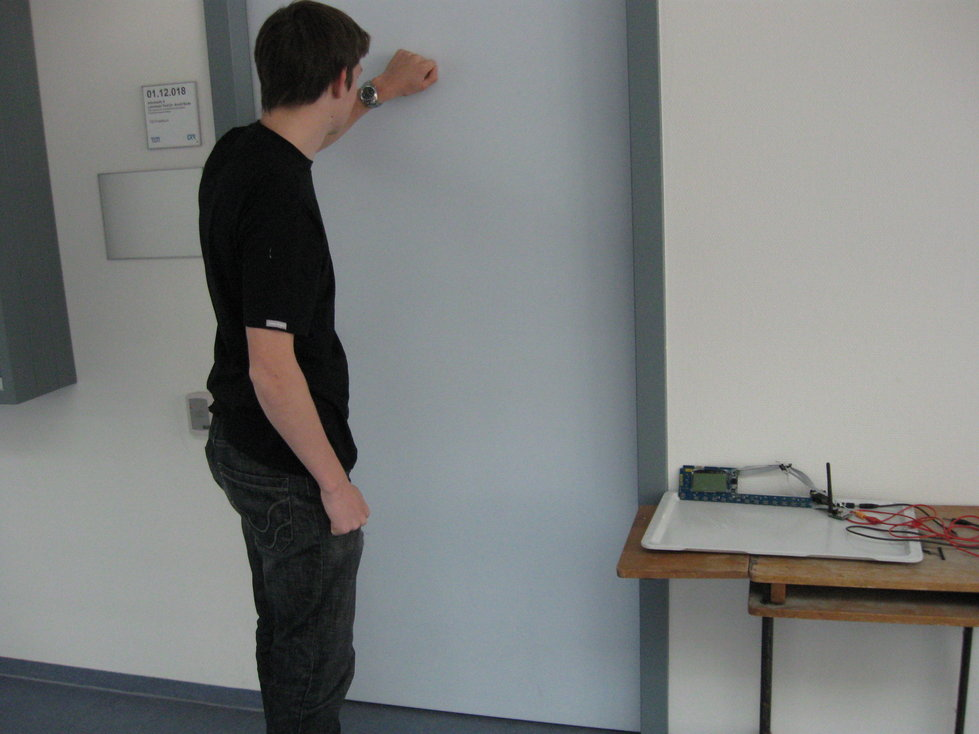
\includegraphics[scale=0.4]{media/story/1.JPG}
    \pause
    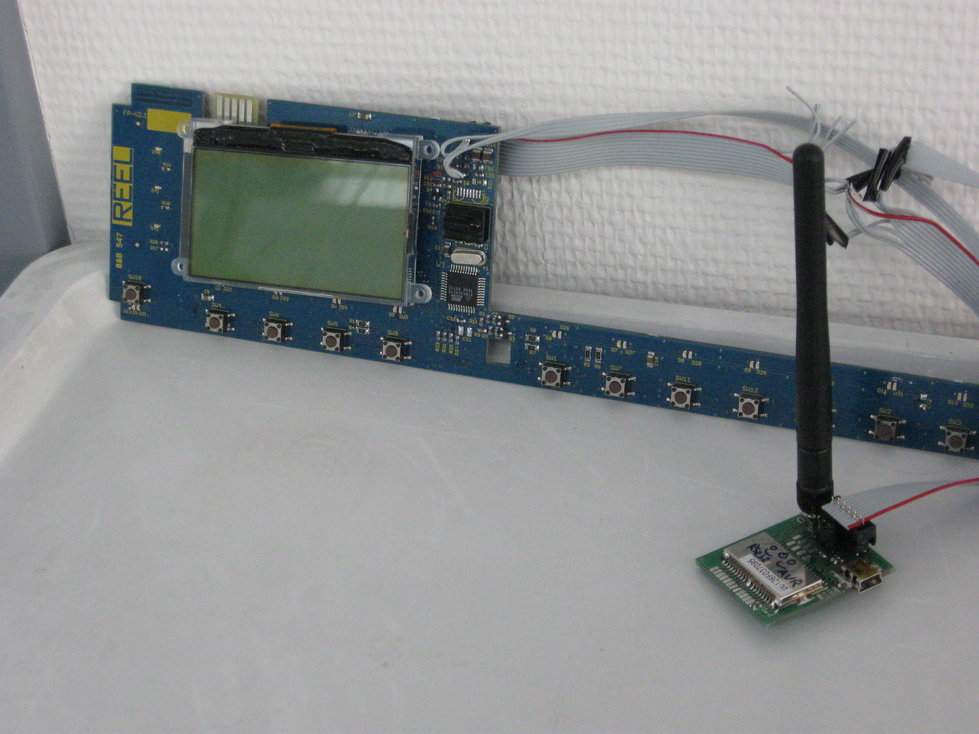
\includegraphics[scale=0.4]{media/story/2.JPG}\
    \pause
    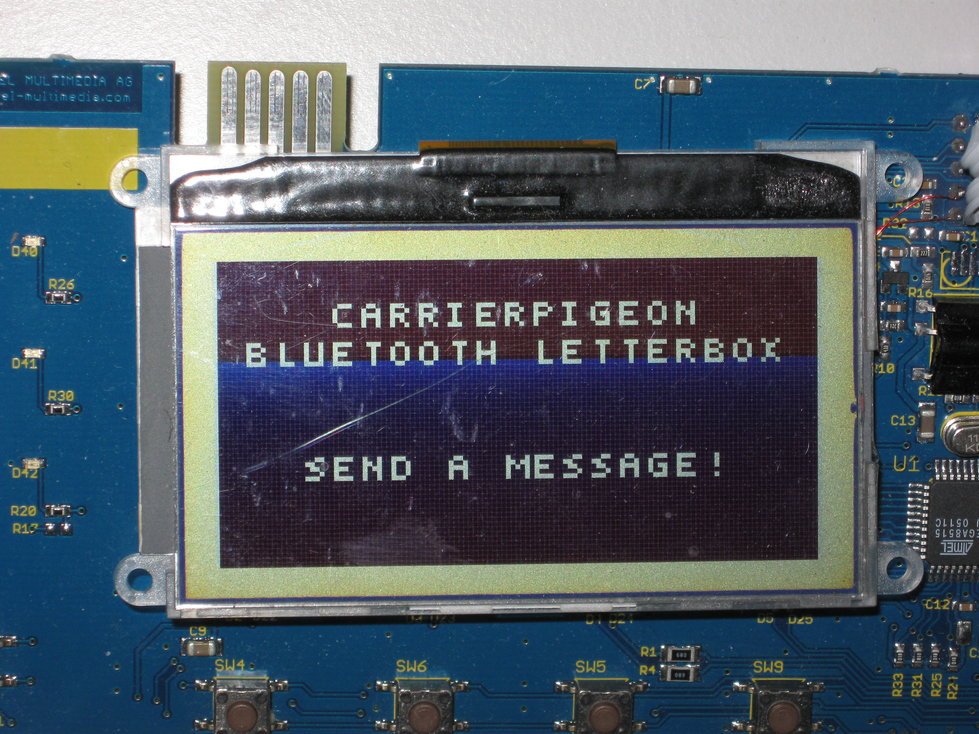
\includegraphics[scale=0.4]{media/story/3.JPG}
    
    
    %[pausesections] <- does not work....

}

\frame{
    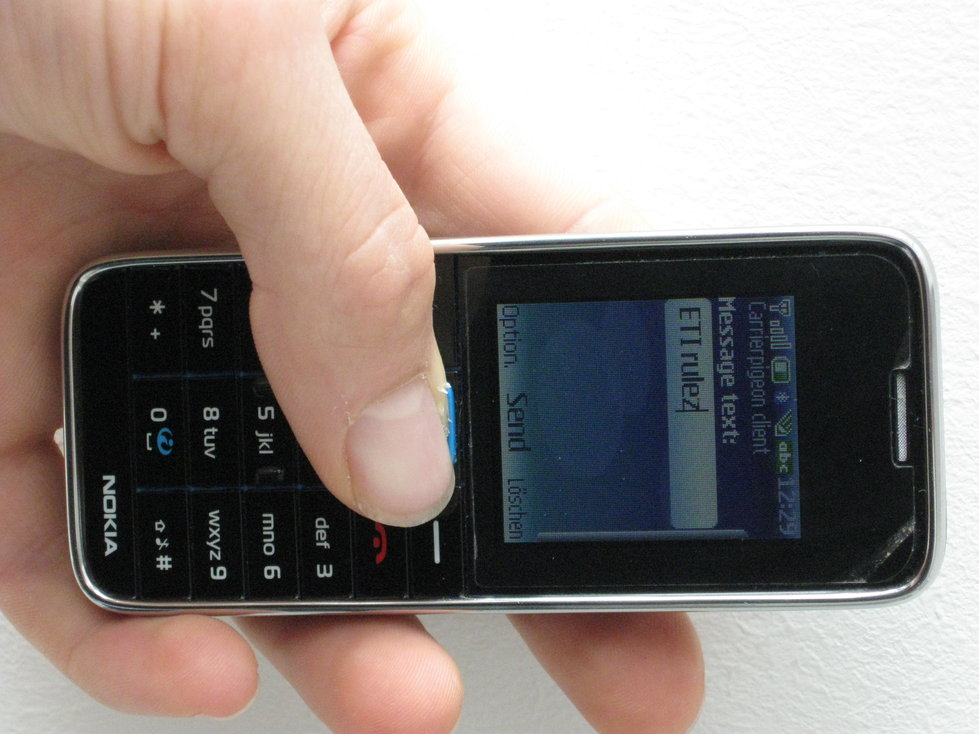
\includegraphics[angle=90, scale=0.5]{media/story/4.JPG}
    \pause
    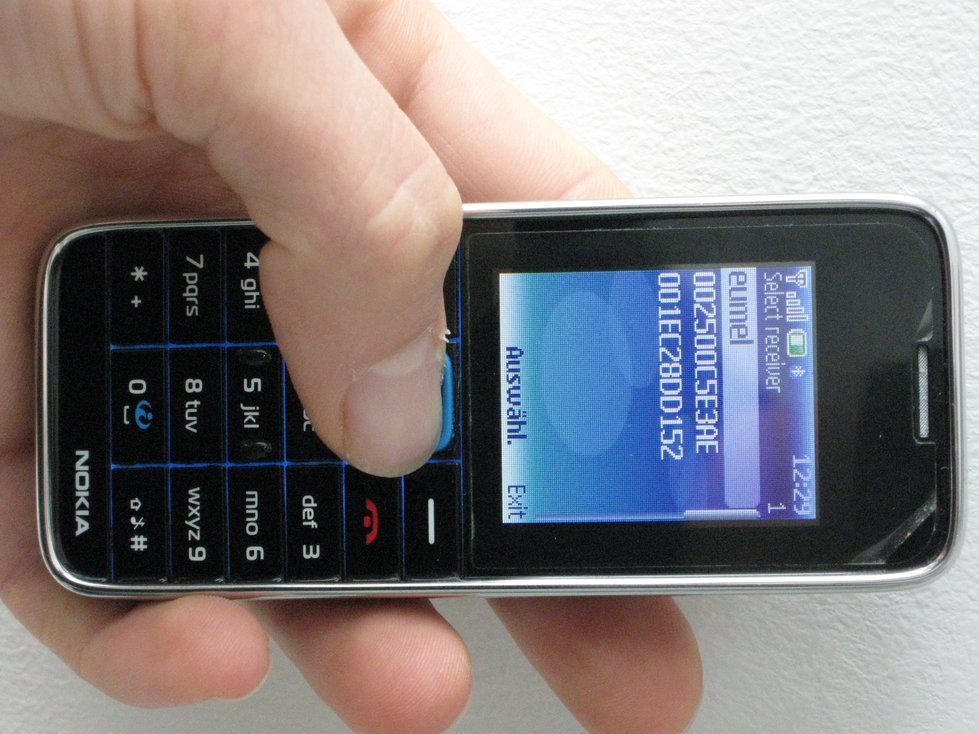
\includegraphics[angle=90, scale=0.5]{media/story/5.JPG}
    
    
}

\frame{
    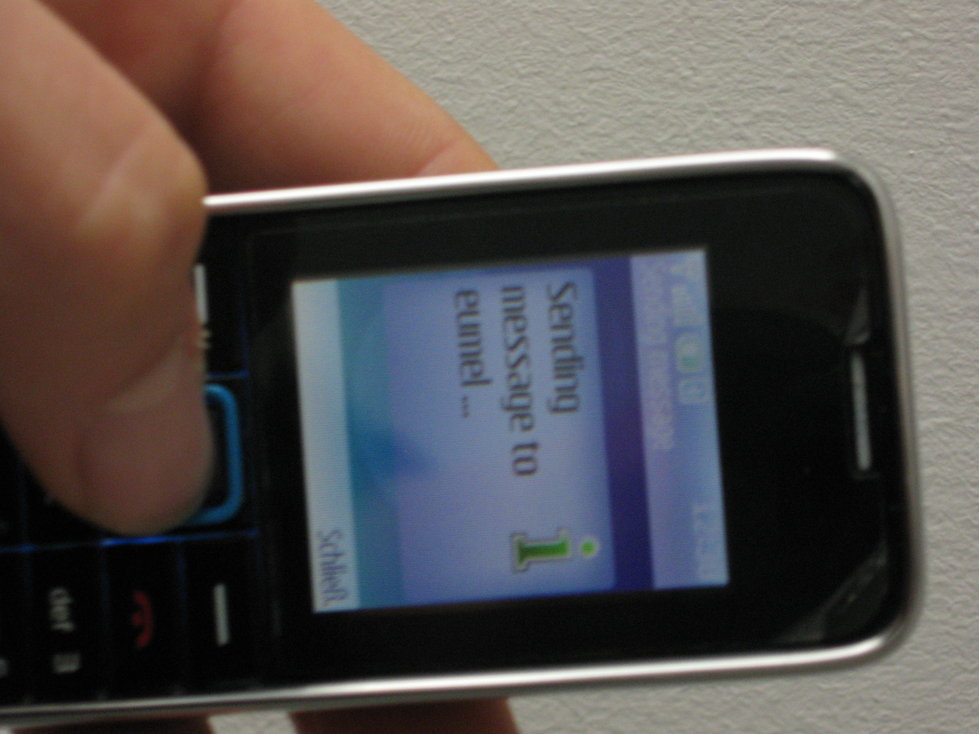
\includegraphics[angle=90, scale=0.5]{media/story/6.JPG}
    \pause
    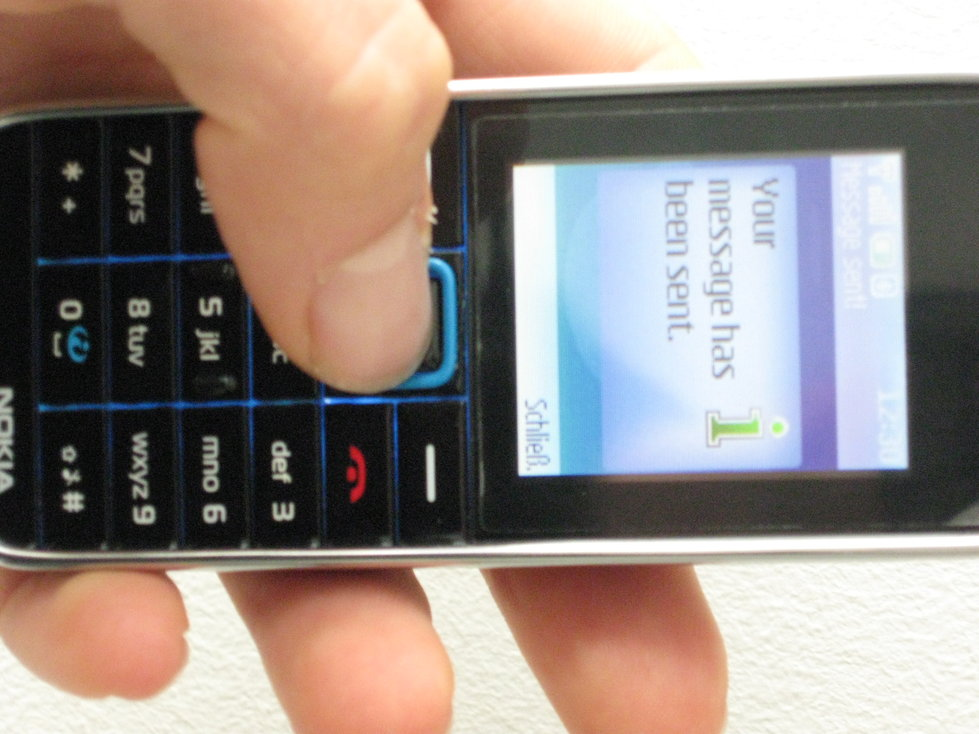
\includegraphics[angle=90, scale=0.5]{media/story/7.JPG}
}

\frame{
    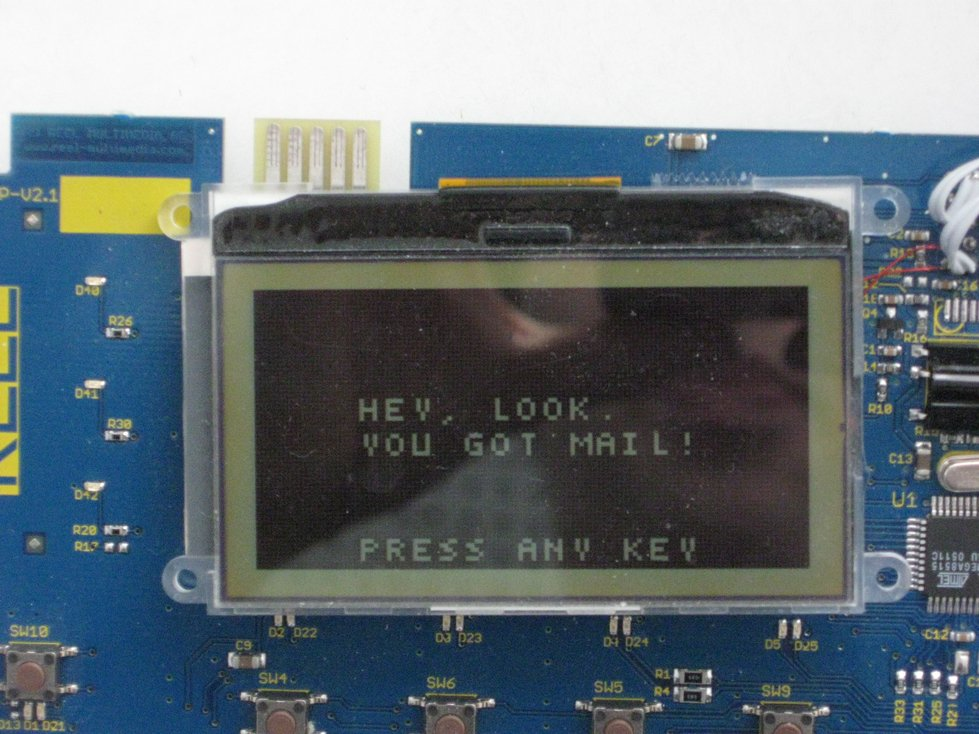
\includegraphics[scale=0.2]{media/story/8.JPG}\
    \pause
    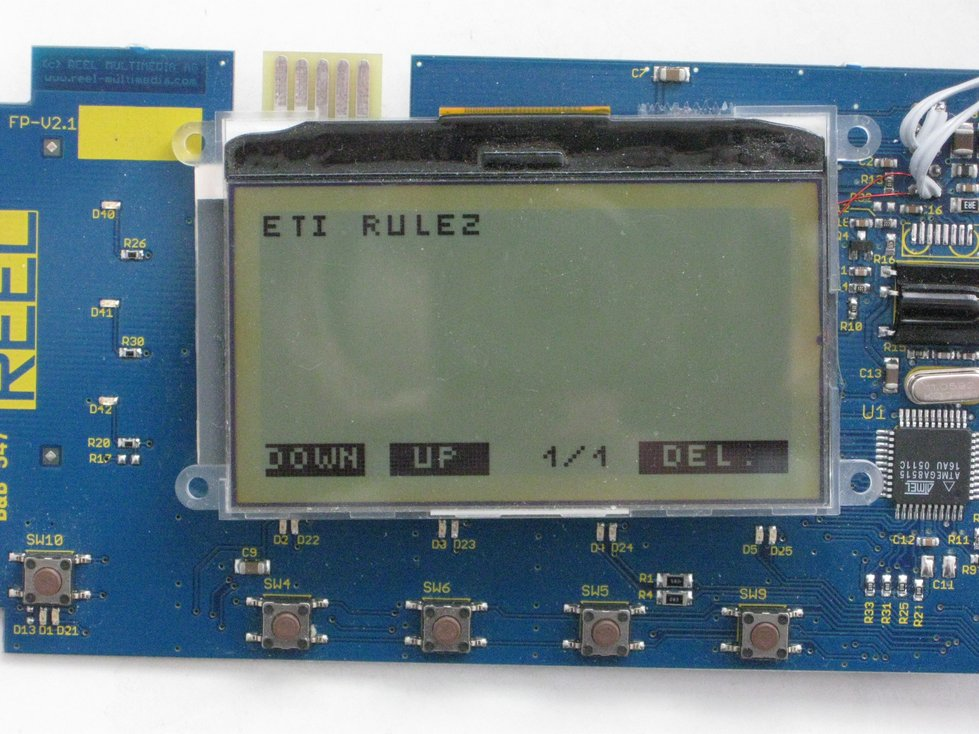
\includegraphics[scale=0.2]{media/story/9.JPG}\
}

\frame{

    \frametitle{Architektur}
    
}

\frame{

    \frametitle{Lösungswege}

}

\frame{

    \frametitle{Sicherheit und Stabilität}

    
\includegraphics[scale=0.4]{media/bluescr}

}

\frame{

    \frametitle{Herausforderung: Stabilität}

}

\frame{
    \frametitle{Herausforderung: Stabilität}

    \begin{itemize}
        \item Server behält Kontrolle 
        \item Timeouts
        \item Vermeidung globaler Variablen
        \item While-Schleifen sorgfältig überprüfen
    \end{itemize}

}

\frame{

    \frametitle{Herausforderung: sicheres Einschalten}

}

\frame{
    
    \frametitle{Herausforderung: sicheres Einschalten}

}



\frame{

    \frametitle{Fazit}

}

\frame{

    % empty
}


%
% --------------------------

\frame{

    \frametitle{Toolchain}

}

\frame{

    \frametitle{Literatur}

}

\end{document}

